% Paper 3 — What Makes a Scientific Question Succeed?
% Compile with: pdflatex paper3.tex  (run twice for references/links)
% Figures are expected in ../results/figures/ (see \graphicspath below).

\documentclass[11pt]{article}

\usepackage[a4paper,margin=1in]{geometry}
\usepackage[T1]{fontenc}
\usepackage[utf8]{inputenc}
\usepackage{lmodern}
\usepackage{microtype}
\usepackage{amsmath,amssymb}
\usepackage{booktabs}
\usepackage{graphicx}
\usepackage{caption}
\usepackage{xcolor}
\usepackage{enumitem}
\usepackage[colorlinks=true,linkcolor=blue!50!black,urlcolor=blue!50!black,citecolor=blue!50!black]{hyperref}

\graphicspath{{../results/figures/}{figures/}}

\newcommand{\addressedrate}{52.7\%}

\title{\bfseries What Makes a Scientific Question Succeed?\\[0.4em]
\large Predicting Future Attention, Resolution, and Premise Revision\\
from Question Structure and Evidence Context\thanks{Third in a series on
temporally grounded evaluation of scientific question discovery; see
\cite{paper1} and \cite{paper2}. Dataset, code, labels, and judge rationales
are public (Reproducibility).}}
\author{Hui Mao\\[0.3em]
\normalsize Independent Researcher\\
\normalsize \texttt{hui.mao@alumni.upenn.edu}\\
\normalsize ORCID: \href{https://orcid.org/0009-0006-7249-4240}{0009-0006-7249-4240}}
\date{}

\begin{document}

\maketitle

\begin{abstract}
\noindent
Large language models are increasingly asked to propose ``important open
questions'', and are typically evaluated by asking another model how good
those questions feel. We replace taste with history. We construct a
temporally grounded dataset of \textbf{980 astronomy research questions}
frozen at five historical cutoffs (2012--2020), spanning eight subfields
and four distinct generation sources --- evidence-tension mining, direct
LLM elicitation, author-stated future work, and weak/negative controls ---
on top of the complete arXiv astro-ph metadata record (\textbf{313{,}189
papers, 2005--2025}). Each question carries a six-group cutoff-time
feature record (text structure, evidence context, novelty, falsifiability,
tractability, field environment) and a tiered outcome label derived from
the five years of literature that actually followed. Under a strict,
source-blinded outcome judge, \addressedrate{} of questions were
substantively addressed; negative-control questions were addressed least
(32\%) and direct-LLM questions most (88\%), the latter carrying a
documented parametric-leakage caveat. Interpretable models trained on
2012--2016 cutoffs predict 2020 outcomes at AUC 0.71 and transfer to
entirely held-out subfields at AUC 0.65--0.71. Measured label noise
implies a perfect-oracle ceiling of AUC 0.76 on these labels, so the
model captures 83\% of the attainable range above chance. Across univariate,
controlled, ablation, and stability analyses, the robust predictors of
future attention are \textbf{prior community recognition} (overlap with
pre-cutoff review articles, $\beta = +0.34$, $p < 10^{-4}$), \textbf{the
density of directly related prior evidence} ($\beta = +0.26$), and
\textbf{explicitly stated competing hypotheses} ($\beta = +0.17$) ---
while high entity-specificity predicts \emph{less} and \emph{slower}
engagement under literature-bounded labels. Five of six pre-stated
mechanism hypotheses, including ``evidence tension beats novelty'', are
\emph{not} supported at scale --- a result only visible because the
dataset is large, multi-cutoff, and control-laden. Answering the
structural-prior question posed by Paper 2's outlook, we further show
that within the tension-mined subset the generating evidence-graph
structure itself is predictive: breadth of the paper cluster in tension
predicts uptake ($\beta=+0.45$/SD), explicit contradiction predicts
engagement, and quantified, cutoff-persistent tensions carry every
resolution and premise refutation --- a learnable, mining-time prior
for structure-first question generation. Finally, a complete replication
of the protocol in a maximally distant second domain --- anti-aging
skincare-ingredient research (19{,}193 PubMed abstracts, 1{,}043
backtested questions, a deterministic template generator and a
checkable-condition judge) --- reproduces the predictability (AUC
0.75--0.84), the control ordering, the breadth effect, the hypothesis
failures, and the reliability ceiling ($\kappa=0.22$ vs.\ 0.21), while
the sign of specificity reverses exactly as the engagement-cost account
predicts. All data, code, labels, and
judge rationales for both domains are released.
\end{abstract}

\section{Introduction}

How scientific attention gets allocated is a central concern of the science
of science, and it has been answered almost entirely at the level of papers
and careers: which combinations of prior work earn citations
\cite{uzzi2013}, which research strategies scientists actually adopt
\cite{foster2015}, how impact is distributed across a field and a lifetime
\cite{fortunato2018,wang2021}. The unit that precedes all of these --- the
research question itself, the bet placed before any paper exists --- has no
comparable empirical treatment. The obstacle is not interest but
measurement: questions leave no bibliographic record, so there is nothing to
attach an outcome to.

This paper constructs those outcomes. We freeze research questions at
historical cutoffs using only the literature available at the time, then
read off what the following five years of literature did with each one. The
resulting dataset makes a question-level analogue of the science-of-science
program possible: rather than asking which papers were cited, we ask which
\emph{questions} the community took up, resolved, or overturned, and which
of their cutoff-time properties predicted that.

The same construction answers a second, narrower question that motivated the
series. Machine-generated research questions are currently evaluated by LLM
or expert panels scoring ``importance'' and ``novelty'' at generation time
--- a measurement of how a question \emph{sounds}, not of what it
\emph{does} \cite{si2024}. Paper 2 of this series~\cite{paper2} introduced
historical backtesting as the alternative: freeze questions using only
pre-cutoff literature, then
observe what the scientific community actually did afterwards. Its
sealed v1.1 release has since grown from a ten-question pilot into a
benchmark family --- a scaled 424-question baseline instance, a
four-cutoff temporal stress test (798 judged questions, 2010--2024), and
a prospective instance frozen in 2026 --- but its unit of comparison
remains the generating \emph{system}: it measures which generator
families produce questions the future engages, not which measurable
properties of an individual question predict that engagement. That
predictor-discovery problem is this paper's subject.

This paper turns the backtesting protocol into a supervised-learning
problem at scale. Three design decisions matter:

\begin{enumerate}
  \item \textbf{The unit of data is (question, cutoff, subfield, source),
    not the question alone.} We generate questions at five rolling
    cutoffs (2012--2020) in eight astronomy subfields, so that one study
    contains what would otherwise be forty historical experiments, and
    era- or field-specific accidents can be detected rather than
    absorbed.
  \item \textbf{No single generator.} Predictors learned from one
    generation system risk being that system's stylistic fingerprint. We
    use four sources --- our evidence-tension system, a direct-LLM
    baseline, questions extracted from the authors' own future-work
    statements, and deliberately weak controls (random claim pairings,
    vague, untestable, and evidence-free-contrarian questions). Without
    negative controls a model can only learn that ``question-shaped
    sentences succeed''.
  \item \textbf{Prediction is out-of-time or out-of-domain, always.}
    Random splits would place near-duplicate questions from the same era
    and topic on both sides. We train on 2012--2016 cutoffs, validate on
    2018, test on 2020, and additionally hold out entire subfields.
\end{enumerate}

The contribution is deliberately not a leaderboard number. It is a
temporally grounded dataset of scientific questions with subsequent
outcomes, and an analysis of \emph{which properties of a question and its
evidence context} predicted future scientific attention, resolution, and
premise revision --- with controls for field popularity, instrument eras,
and generation method, and with stability checks across cutoffs,
subfields, and sources.

\section{Related work}

\subsection{Problem choice in the science of science}

The choice of research problem is treated in this literature as a strategic
act under uncertainty. Foster, Rzhetsky and Evans~\cite{foster2015},
analysing millions of MEDLINE abstracts, showed that scientists
overwhelmingly pursue conservative strategies --- deepening established
chemical relationships rather than bridging distant ones --- and that this
conservatism is individually rational while collectively suboptimal, a
finding later formalised as a question of how a field should allocate its
collective search~\cite{rzhetsky2015}. Uzzi et al.~\cite{uzzi2013} reached a
compatible conclusion from the citation side: the highest-impact papers
combine a conventional core with a tail of novelty, so novelty by itself is
not the operative virtue. Fortunato et al.~\cite{fortunato2018} survey the
broader program, and Wang and Barabási~\cite{wang2021} give it book-length
treatment.

Our results speak directly to this line. The predictor we find strongest ---
prior recognition of a question in review articles --- is a question-level
measurement of exactly the conservatism Foster et al.\ document at the level
of research strategy, and our null result for semantic novelty is what Uzzi
et al.'s conventionality finding would predict. The contribution is the unit
of analysis: this literature observes what scientists \emph{did} and infers
the strategy, whereas we fix the candidate questions in advance and observe
which were taken up. Because the questions are frozen before the outcome
window opens, and because deliberately weak controls are included, the
design separates properties of a question from properties of the field it
sits in.

\subsection{Generating and evaluating research questions}

Machine generation of research questions and hypotheses has a long lineage,
from literature-based discovery~\cite{swanson1986} to LLM systems that
propose ideas or run entire studies~\cite{lu2024,wang2024,baek2024}, and it
has been argued that question-asking is itself a core capability on the path
to more general scientific intelligence~\cite{kitano2021}. Evaluation has
not kept pace. The most rigorous instance of the dominant paradigm, Si et
al.'s expert study~\cite{si2024}, still measures opinion at generation time
rather than what the ideas turned out to be worth. Outcome-based
alternatives have appeared only recently and independently:
HindSight~\cite{hindsight2026} matches generated ideas against papers
published after a temporal cutoff and finds that LLM-judged novelty
correlates \emph{negatively} with realised impact, and the
ideation--execution study~\cite{ideationgap2025} had human researchers
execute both LLM and human ideas, finding that the LLM ideas rated higher
before execution scored lower after it. Both converge with our null results
for novelty from different fields and different methods.

Paper 1~\cite{paper1} built an evidence-graph system that generates
questions from cross-paper observational tensions. Paper
2~\cite{paper2} defined the backtesting benchmark and showed, in its
pilot, that future literature substantively
engaged all ten frozen exoplanet-atmosphere questions (one premise ---
a strongly subsolar water abundance for HD~209458\,b --- later refuted
by three independent analyses, the exact convergence the question
called for). Its sealed v1.1 release then scaled the evaluation and
sharpened three findings this paper builds on. First, at $n=125$ per
baseline, engagement rates discriminate between generator families
(random templates 73\% vs.\ direct-LLM 96\%, $p<10^{-4}$), and random
templates acquire a measurable 11\%-answered floor --- engagement
metrics have a priced chance level. Second, a generator decomposition
(LLM-only vs.\ deterministic evidence structure vs.\ structure-plus-LLM
verbalization) crossed with a four-cutoff temporal stress test
(2010--2024, 798 judged questions, the last window postdating the
model's training) located the foresight signal in \emph{pre-cutoff
evidence structure} rather than model weights: LLM-only generation
shows near-ceiling engagement and the closest phrasing to future
literature at every cutoff, yet an answered rate indistinguishable from
random templates and no premise refutations outside the deepest-history
era. Third, a seven-rater agreement study (two blinded humans, five
judge models, 90 items) found the two humans agree at only
$\kappa=0.17$ --- indicting the outcome taxonomy, not any particular
judge, and capping what absolute outcome rates can mean. Both papers
evaluate question \emph{generators}; neither learns question-level
predictors, which is the question this paper addresses: \emph{what,
measurably, makes a question one the community will take up?}

\subsection{Outcome labels and judge reliability}

Scoring a strategy on held-out history is standard in quantitative finance,
along with its documented failure mode --- overfitting to the backtest
itself~\cite{bailey2014} --- which motivates the freezing rules we inherit;
forecasting benchmarks apply the same logic to events resolving after
training~\cite{zou2022}, and SWE-bench~\cite{jimenez2024} showed how frozen
data plus a fixed task format can reorganise a field around measurable
progress.

Because our outcome labels are assigned by a language model, their
reliability is itself a measured quantity rather than an assumption. Using
LLMs as judges is now routine~\cite{zheng2023}, and so is certifying them by
agreement with other models --- a practice Paper 2's seven-rater study shows
to be badly optimistic: on an analogous taxonomy two independent human
annotators agreed at $\kappa = 0.17$, below every model--model pair. We
therefore report agreement with the conventional interpretive
benchmarks~\cite{landis1977} attached, treat all absolute rates as
rater-relative, and hold the judge fixed within every comparison.

To our knowledge no prior dataset attaches future-outcome labels to
\emph{questions} frozen at multiple historical cutoffs with controlled
generation sources and negative controls.

\section{Theoretical framework}
\label{sec:theory}

Why should any property measurable at the cutoff predict what a scientific
community subsequently does with a question? The empirical sections that
follow are organised by a single account --- \emph{attention allocation as
recognition-constrained foraging} --- assembled from three premises, each
with independent support in prior literature. We are explicit about its
epistemic status at the end of the section: the account was articulated to
organise this paper's results, not derived before them, and its falsifiable
content is therefore prospective.

\paragraph{Premise 1: evaluation is the price of attention.} A community's
capacity to take up questions is bounded by researcher time, instrument
access, and career risk. Before anyone invests in a question, someone must
pay an evaluation cost: deciding whether it is well posed, whether it can
be answered with accessible data, and whether an answer would be
publishable. Bounded rationality~\cite{simon1955} implies this cost is not
paid exhaustively --- it is avoided wherever a cheaper proxy exists.

\paragraph{Premise 2: prior recognition amortises the evaluation cost.}
Signals that the community has already evaluated a question --- above all
its appearance in a review article --- let an individual researcher skip
the evaluation and inherit its conclusion. This is cumulative
advantage~\cite{merton1968} operating at the level of questions rather
than of people or papers: a recognised question gets re-recognised,
because recognition is itself the cheapest available evidence of worth.
Foster, Rzhetsky and Evans' finding that scientists overwhelmingly choose
conservative, tradition-following research strategies~\cite{foster2015} is
the strategy-level face of the same economy.

\paragraph{Premise 3: researchers forage on cost-and-yield cues.}
Information-foraging theory~\cite{pirolli1999} models an information
seeker as following ``scent'' toward patches of high expected yield per
unit cost. Read as foraging cues, the feature groups of
Section~\ref{sec:features} make differentiated predictions. A dense base
of directly related prior evidence signals a rich patch in which existing
tools, data, and comparison points apply, lowering the marginal cost of a
contribution --- whether or not that evidence is in tension. An explicitly
articulated pair of competing hypotheses converts an open-ended evaluation
problem into a designable discriminating study, lowering execution cost.
Semantic novelty, by contrast, raises evaluation cost without lowering
execution cost. And entity-specificity shrinks the set of researchers for
whom the patch is cheap at all.

\medskip
\noindent Together the premises order the predictors the paper tests:

\begin{enumerate}[label=(P\arabic*)]
  \item prior recognition in reviews should be the strongest and most
    stable positive predictor of five-year attention;
  \item density of directly related evidence should predict uptake
    independently of whether that evidence agrees --- density, not
    tension;
  \item explicit competing hypotheses should predict engagement and,
    conditional on engagement, resolution;
  \item semantic novelty should be null to weakly positive at a five-year
    horizon --- the question-level analogue of the finding that impact
    favours conventional cores~\cite{uzzi2013};
  \item entity-specificity should predict less and slower
    \emph{measured} attention.
\end{enumerate}

Two boundaries of the account deserve emphasis. First, it is a theory of
where attention flows, not of what a question is worth; the discussion
returns to the gap between the two, and the error analysis of
Section~\ref{sec:robustness} exhibits it concretely --- the attention
model's largest miss is a question the community engaged by overturning
its premise. Second, the account does not cover the premise-refutation
channel at all. Refutation is error-correction rather than
attention-following: Section~\ref{sec:structureprior} finds it
concentrated in quantified, recurrent contradictions --- structures that
persist across cutoffs until someone runs the decisive test. A foraging
account predicts the crowd's path; it is silent about which accepted
conclusion will fall.

Finally, the epistemic status. The six hypotheses of
Section~\ref{sec:models} were stated before the outcomes were known; this
framework was assembled afterwards, as the interpretation the results
select among prior theories --- Merton's cumulative advantage, Foster et
al.'s conservatism, Uzzi et al.'s conventionality, and the foraging model
of information seeking. Its falsifiable content is prospective:
transported to a new domain, it predicts that recognition and evidence
density transfer as predictors while novelty remains null, and the frozen
prospective instance of~\cite{paper2} puts that prediction on the record
before the outcomes exist.

\section{Dataset construction}

\subsection{Corpus}

We harvested the complete arXiv astro-ph metadata record --- titles,
abstracts, submission dates, and categories --- from 2005-01 through
2025-12 via the public arXiv API (\textbf{313{,}189 papers} after
deduplication; \texttt{pipeline/harvest.py}). Papers are assigned to
eight subfields by transparent weighted keyword rules over
title+abstract (multi-membership allowed): exoplanet atmospheres (4{,}354
papers), protoplanetary disks (10{,}378), stellar activity (4{,}347),
fast radio bursts (1{,}966), gravitational waves (17{,}989), galaxy
evolution (21{,}390), cosmology tensions (16{,}403), and compact objects
(34{,}266). The classifier is identical at every cutoff, so subfield
corpora are time-sliced views of a fixed rule, not retrofitted topic
models.

Each cutoff year $c \in \{2012, 2014, 2016, 2018, 2020\}$ defines a
\textbf{past window} $[c-7,\, c]$ used for generation and features and a
\textbf{future window} $(c,\, c+5]$ used only for labels. The five future
windows all close by 2025-12-31, giving every cutoff the same 5-year
outcome horizon.

\subsection{Question generation (40 cells $\times$ quota 25)}

For every (cutoff, subfield) cell:

\begin{itemize}
  \item \textbf{Evidence-tension (10).} We mine the cell's past-window
    abstracts for tension statements (contradiction, discrepancy,
    unexplained-result markers), cluster them so that each cluster spans
    $\geq 2$ distinct papers, and have an LLM phrase each cluster as one
    precise question grounded only in the mined sentences. Provenance
    (exact sentences, arXiv ids, dates) is stored with the question.
  \item \textbf{Direct LLM (5).} The baseline the field implicitly uses:
    the model sees a year-stratified sample of pre-cutoff titles and is
    asked for the most important unanswered questions, with an explicit
    knowledge-freeze instruction.
  \item \textbf{Future-work (5).} Sentences in which pre-cutoff authors
    themselves flag an open problem (``remains poorly constrained'',
    ``further observations are needed''), selected for topic diversity
    and converted faithfully into interrogative form. These are real
    scientists' questions.
  \item \textbf{Controls (5).} Two random claim-pairings across unrelated
    papers, one vague question, one untestable question, one
    evidence-free consensus challenge --- all phrased by the same LLM so
    that surface style cannot separate controls from real candidates.
\end{itemize}

Near-duplicates within a cell are removed (TF--IDF cosine $\geq 0.75$).
The ten frozen Paper 1 evidence-graph questions join the dataset as a
small additional source (cutoff 2020, exoplanet atmospheres), linking
this study to the original system.

\textbf{Realized totals: 980 questions} --- 374 evidence-tension, 200
direct-LLM, 196 future-work, 200 controls, 10 Paper 1. Every non-FRB cell
filled its full quota of 25; early fast-radio-burst cells are
data-limited by history itself (the pre-2013 FRB literature contains 21
papers, yielding 11 questions at the 2012 cutoff), which we treat as a
feature of honest backtesting rather than a defect. The dataset is
regenerable bit-identically from the frozen LLM cache; rebuilding the
corpus from scratch and regenerating produced byte-identical questions.

Temporal isolation is enforced by construction --- every mined sentence
and every title shown to a generator predates the cutoff --- and verified
by an automated validator over the frozen records (980/980 pass).

\subsection{Feature record (six groups, all cutoff-time)}
\label{sec:features}

\begin{description}
  \item[A. Text structure] length, named entities, numbers, causal /
    comparative / mechanistic language, measurable quantities, explicit
    alternatives (``real or artifact''), falsification wording, yes/no
    form, and a composite specificity score.
  \item[B. Evidence context] retrieval of the top-20 pre-cutoff subfield
    papers for each question: similarity mass (top-1, mean top-5, count
    above threshold), instrument diversity among retrieved papers,
    density of tension markers in the retrieved evidence, and the age
    profile of that evidence; plus native evidence-record features
    (paper count, year spread) for tension-sourced questions.
  \item[C. Novelty] nearest-neighbour semantic distance to the
    pre-cutoff corpus, mean top-10 similarity, concept-pair novelty (do
    the question's two most distinctive terms co-occur in any pre-cutoff
    paper?), and overlap with pre-cutoff review articles (was the
    question already posed in reviews?).
  \item[D. Falsifiability / answerability] rule-based markers plus a
    blinded LLM structured coding of \{observable, competing hypotheses,
    quantitative test, falsification path\} for every question.
  \item[E. Tractability] facilities named in the question checked
    against a lexicon of $\sim$50 astronomical facilities with
    operational epochs: counts of already-operational vs.\ future
    instruments, archival-data markers, longitudinal / theory /
    large-sample requirements.
  \item[F. Field environment (controls)] subfield publication volume and
    growth at the cutoff, review activity, share of all astro-ph output,
    and proximity of the subfield's next major facility launch (capped
    at 10 years). These are confounders to control for, not virtues of
    the question: without them a model mistakes hot fields for good
    questions.
\end{description}

\subsection{Tiered outcome labels}

\textbf{Tier 1 (automatic candidates).} For each question we retrieve
future papers from its subfield's future window: relevant-paper count
(cosine $\geq 0.18$), weak-relevance count, first-follow-up date, lead
time in months, and review recognition.

\textbf{Tier 2 (strict, blinded LLM judge).} For every question with any
plausible future evidence (956 of 980; the rest are auto-labeled
\texttt{not\_addressed}), a GPT-4o judge sees the question and its top-8
retrieved future records --- never the generation source. The rubric is
deliberately strict and two-stage: the judge first classifies every
candidate paper as \textbf{direct} (investigates this question's own
objects, quantities, or claimed relationship), \textbf{adjacent} (same
topic only), or unrelated, and only then assigns \texttt{addressed},
\texttt{answer\_status} $\in$ \{answered, partially\_addressed,
posed\_but\_open, premise\_refuted, not\_addressed\},
\texttt{premise\_status}, supporting ids, a rationale, and a confidence.
\texttt{addressed} is \emph{derived}: it requires at least one direct
candidate. This rubric matters --- a first-pass lenient judge
(GPT-4o-mini, same evidence) called 94\% of questions addressed by
accepting topical overlap; the strict per-candidate rubric brings the
rate to \addressedrate{} and restores variance to every analysis
downstream.

\textbf{Tier 3 (independent verification).} A second model (GPT-4o-mini)
re-judges all premise\_refuted cases plus a 20\% random sample under the
identical rubric ($n=200$): raw agreement on \texttt{addressed} is 63.5\%
($\kappa = 0.21$), status agreement 58.4\% ($\kappa = 0.22$). The
disagreement is one-directional --- the weaker model is systematically
more lenient, almost never the reverse (its ``partially\_addressed''
precision against the strict judge is 0.99) --- so we treat the strict
labels as primary and release both, with all rationales and supporting
ids, for audit. These $\kappa$ values sit exactly at the measurement
ceiling Paper 2 v1.1 established for outcome taxonomies of this kind:
in its seven-rater study, two independent, careful human annotators
agreed at only $\kappa=0.17$, and every judge model matched a
professional annotator about as well as the humans matched each other
($\kappa=0.17$--$0.26$). We therefore adopt Paper 2's reporting
discipline: absolute rates are rater-relative, and every comparative
claim in this paper is made under a single fixed judge.

\subsection{Design of the retrieval and judging stages}
\label{sec:pipeline}

The two information-access components deserve fuller specification.

\paragraph{Retrieval.} Both the cutoff-time evidence features and the
future-window label candidates use the same retriever: TF--IDF over
title-plus-abstract with English stop-word removal, a 50{,}000-term
vocabulary, and sublinear term-frequency scaling, fitted separately
within each (subfield, window) corpus, with cosine ranking. Three
properties motivate this deliberately classical choice over neural
embedding retrieval. First, \emph{temporal safety}: the cutoff-time
retriever may see nothing newer than the cutoff, and a term-statistics
model fitted on the past window satisfies this by construction, whereas
any pretrained embedding model carries post-cutoff language in its
weights --- the retrieval-side twin of the parametric-leakage channel
documented for generation. Second, \emph{determinism and auditability}:
term weights are inspectable, every ranking reproduces exactly from the
frozen corpus manifest, and no model version enters the provenance
chain. Third, a \emph{conservative bias with a known direction}:
term-based retrieval under-matches paraphrase, which pushes labels
toward \texttt{not\_addressed}; we prefer an engagement floor whose
direction is known to an unquantified error, and the
threshold-starvation curve of Section~\ref{sec:robustness} makes the
bound explicit. The cost --- missed semantic matches, most severe for
narrow object-level questions --- is measured rather than hidden, via
the imported evidence-graph questions of Section~\ref{sec:robustness}
and the specificity results.

\paragraph{Judging.} For each question with any plausible future
evidence (top-1 similarity above threshold; 956 of 980, the remaining 24
auto-labelled \texttt{not\_addressed}), the judge receives the
question, its cutoff date, and the top-8 retrieved future records ---
never the generation source. The rubric is two-stage per candidate
before any outcome is assigned: each record is classified
\emph{direct} (investigates this question's own objects, quantities, or
claimed relationship), \emph{adjacent} (same topic only), or unrelated,
with topical similarity explicitly insufficient for \emph{direct};
\texttt{addressed} is then derived, requiring at least one direct
candidate, after which the five-way status, premise status, supporting
ids, a written rationale, and a confidence are recorded. All calls run
at temperature~0 against a pinned model version and are cached, so the
released labels regenerate exactly; rationales and supporting ids are
released for audit. Throughout, the judge is treated as a measurement
instrument with a measured error rate rather than as an oracle: its
leniency direction, second-judge agreement, and the ceiling that
agreement implies are quantified in Section~\ref{sec:robustness}.

\section{Models and evaluation protocol}
\label{sec:models}

Baselines before models, interpretable models before ensembles: majority
class; field-popularity-only; question-text-only (bag of words); then L2
and L1 logistic regression, random forest, and gradient boosting on the
structured features; multinomial GBM for the five-way status; a Cox
proportional-hazards model for time-to-first-follow-up; and within-cell
ranking concordance between model scores and future paper counts.

All headline numbers use the \textbf{temporal split} (train 2012--2016,
validate 2018, test 2020). Generalization is probed with
\textbf{leave-one-subfield-out} and a fixed \textbf{cross-domain split}
(train: exoplanet atmospheres, disks, stellar activity, galaxy evolution
$\rightarrow$ test: FRBs, gravitational waves, cosmology tensions,
compact objects). Random splits are not reported anywhere in this paper.

Predictor identification goes beyond feature importance: (i) univariate
associations; (ii) controlled logistic effects with subfield, cutoff,
source, and environment covariates; (iii) feature-group ablations;
(iv) sign-stability of controlled effects across cutoffs, subfields, and
generation sources. A predictor is called robust only if it survives all
four.

\subsection*{Pre-stated hypotheses}

\begin{description}[style=multiline,labelwidth=1.6em,leftmargin=2.2em]
  \item[H1] Cross-source evidence tension predicts future attention
    better than semantic novelty.
  \item[H2] Observation availability predicts short-term attention but
    not premise refutation.
  \item[H3] Explicit competing hypotheses raise the probability of being
    answered, given attention.
  \item[H4] Novelty shows an inverted-U: very high novelty reduces
    short-term attention.
  \item[H5] Field popularity inflates future paper counts without
    raising answer rates.
  \item[H6] High-tension $\times$ high-tractability questions succeed
    most.
\end{description}

\section{Results}

\subsection{What happened to the questions}

Of 980 frozen questions, \textbf{\addressedrate{} were substantively
addressed} within five years of their cutoff: 474 partially addressed,
30 posed-but-open, 8 answered, 4 premise-refuted, 464 not addressed.
Addressed questions drew a mean of 3.8 relevant future papers and were
first engaged after a mean of 16.7 months. Rates are stable across
cutoffs (0.45--0.57), confirming that no single era drives the results.

Generation source separates outcomes exactly as a functioning label
should (Table~\ref{tab:sources}, Figure~\ref{fig:addressed-rates}).

\begin{table}[htbp]
  \centering
  \caption{Addressed rate by generation source (strict blinded judge,
  5-year horizon).}
  \label{tab:sources}
  \begin{tabular}{lc}
    \toprule
    Source & Addressed \\
    \midrule
    Direct LLM                        & 0.88 \\
    Author future-work                & 0.51 \\
    Evidence-tension                  & 0.47 \\
    Weak/negative controls            & 0.32 \\
    Paper 1 evidence-graph ($n=10$)   & 0.20 \\
    \bottomrule
  \end{tabular}
\end{table}

\begin{figure}[htbp]
  \centering
  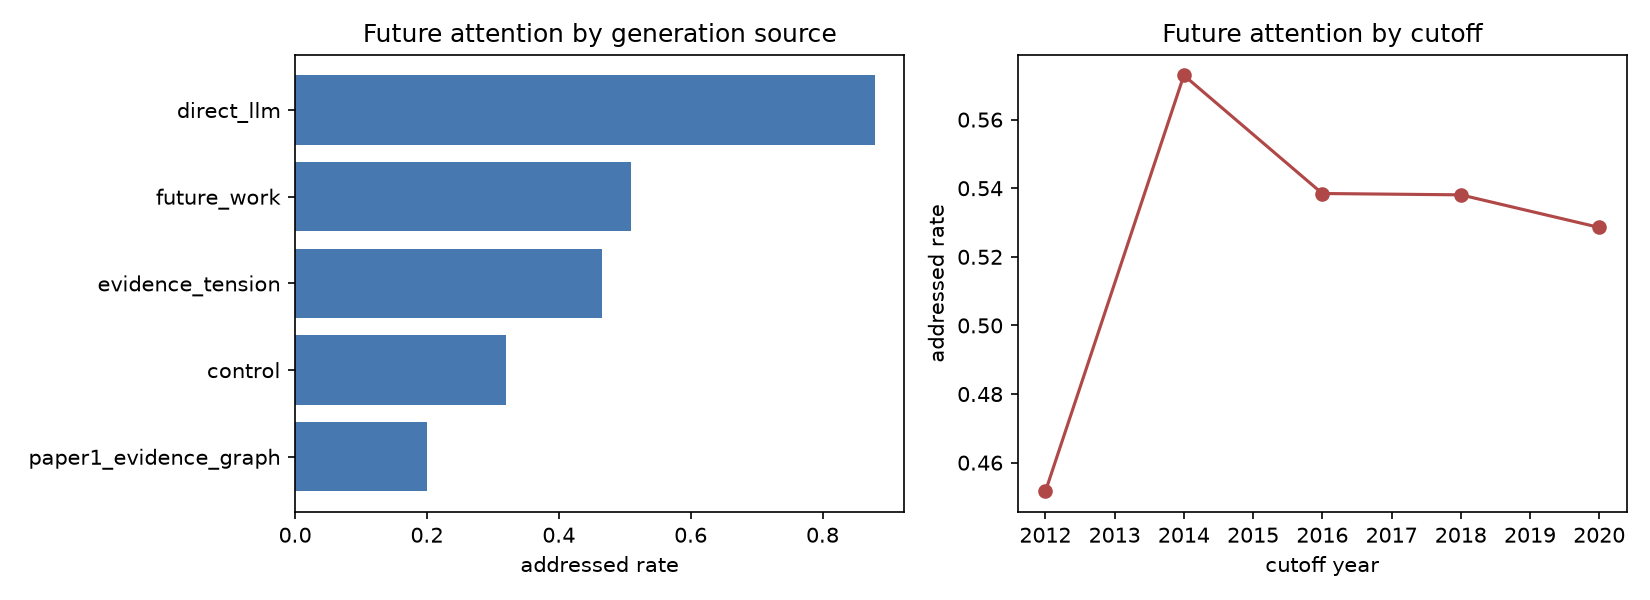
\includegraphics[width=0.85\linewidth]{addressed_rates}
  \caption{Addressed rates by generation source and cutoff.}
  \label{fig:addressed-rates}
\end{figure}

\begin{figure}[htbp]
  \centering
  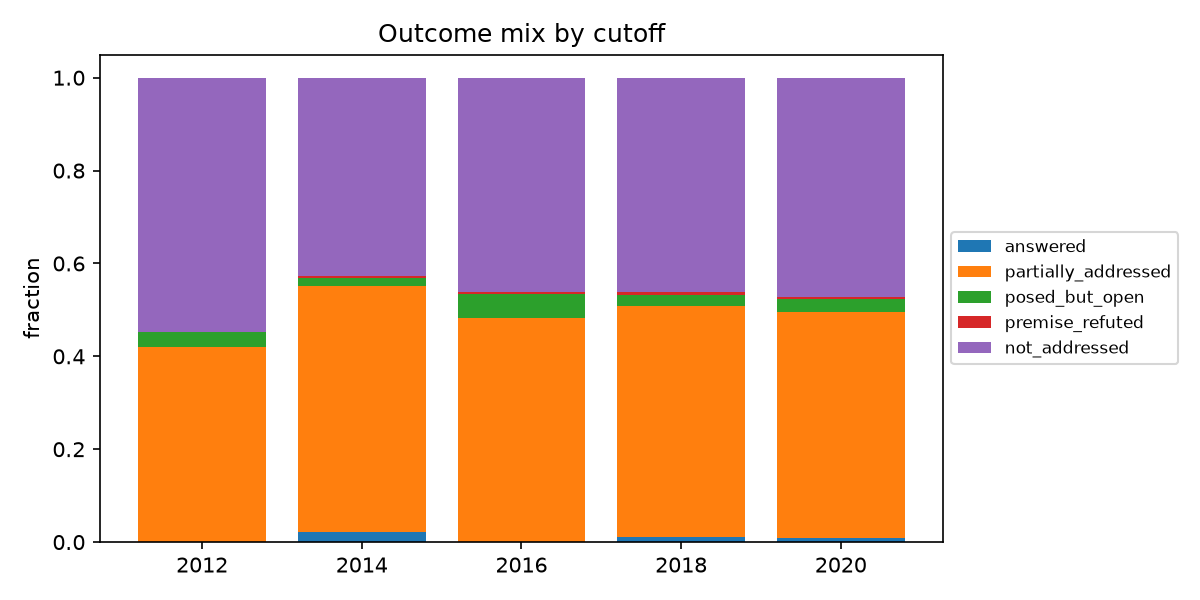
\includegraphics[width=0.85\linewidth]{outcome_mix}
  \caption{Outcome status mix across the 980 frozen questions.}
  \label{fig:outcome-mix}
\end{figure}

Controls land lowest in aggregate --- but the aggregate hides the
dataset's most instructive split (Table~\ref{tab:subtypes}). Random claim
pairings, the purest chance-directed baseline, are addressed at 8.7\%:
that, not the pooled 32\%, is the floor for chance-level engagement.
Vague questions, by contrast, reach 0.850 --- within three points of the
direct-LLM rate and above every mined source --- by being broad enough
that some future paper always qualifies as direct. Coverage-style metrics
are thus not merely gameable in principle; the worst-by-construction
questions in the dataset game them in practice, which is why no
engagement rate in this paper is interpreted without its source
composition, and why the strict-bar analysis of
Section~\ref{sec:robustness} prices breadth explicitly.

\begin{table}[htbp]
  \centering
  \caption{Outcomes within the negative-control arm, by subtype.}
  \label{tab:subtypes}
  \begin{tabular}{lccc}
    \toprule
    Control subtype & $n$ & Addressed & Mean direct papers \\
    \midrule
    Random claim pairing & 80 & 0.087 & 0.17 \\
    Consensus challenge  & 40 & 0.275 & 0.45 \\
    Untestable           & 40 & 0.300 & 0.53 \\
    Vague                & 40 & 0.850 & 2.62 \\
    \bottomrule
  \end{tabular}
\end{table}

The direct-LLM rate of 0.88 should be read with care: the generating model
may know, parametrically, which 2016-era questions became hot topics, an
irreducible leakage channel we document rather than claim to eliminate
(Section~\ref{sec:limitations}). Paper 2 v1.1 measures this channel
directly and finds the same signature at scale: its direct-LLM baseline
has the highest phrasing similarity to future literature of any system,
near-ceiling engagement (96\% at $n=125$), yet an answered rate
statistically indistinguishable from random templates and zero premise
refutations outside the one era its weights could have memorized ---
``memorized relevance without specific foresight''. The mined sources
(tension, future-work) are built from pre-cutoff sentences and cannot
leak this way; that they land at $\sim$0.5 against a strict judge is
the honest base rate of real open problems. The ten Paper 1 questions
--- all engaged by future literature under Paper 2's adjudicated pilot
evaluation (coverage 100\%) --- score only 2/10 here, a direct
measurement of how much this paper's abstract-only retrieval and strict
direct-engagement bar \emph{under-count} engagement for narrow,
object-level questions (they average 3.4 entities per question vs.\ 1.5
elsewhere). Paper 2's own cross-instance anchor shows the same
instrument-dependence from the other side: re-judging its ten questions
on a 2.4$\times$ larger corpus flipped four labels in both directions
--- outcome rates are functions of the (corpus, retriever, judge)
triple, and are comparable only within one instance.

\subsection{Predicting future attention (Task A)}

Temporal split, test = cutoff 2020 ($n=210$, base rate 0.53); results in
Table~\ref{tab:models}.

\begin{table}[htbp]
  \centering
  \caption{Task A (future attention) on the temporal test split.}
  \label{tab:models}
  \begin{tabular}{lcl}
    \toprule
    Model & AUC & Notes \\
    \midrule
    Majority class            & 0.500 & \\
    Field popularity only     & 0.519 & popularity is \emph{not} a question-level predictor \\
    Question text only (BoW)  & 0.772 & absorbs source style + topic hotness \\
    Logistic (structured, L2) & 0.713 & interpretable \\
    Logistic (L1)             & 0.707 & \\
    Random forest             & 0.718 & \\
    Gradient boosting         & 0.688 & \\
    \bottomrule
  \end{tabular}
\end{table}

Three observations. First, everything question-level beats field
popularity by a wide margin: which questions succeed is not just which
fields are hot. Second, raw question text is the strongest single signal
--- but it is also the least meaningful, because it can encode the
generator's stylistic fingerprint (direct-LLM questions are both
stylistically distinctive and 88\% addressed). Third, the structured
features reach AUC 0.71 while being \emph{auditable}: every unit of
signal is a named, cutoff-time property.

\paragraph{Out-of-domain.} Trained on four subfields and tested on four
entirely unseen ones ($n=470$), the structured logistic model holds AUC
\textbf{0.710} (GBM 0.647). Leave-one-subfield-out AUCs span 0.62--0.78
with every subfield above chance (stellar activity 0.78, gravitational
waves 0.75, cosmology 0.71, disks 0.70, exoplanet atmospheres 0.69,
galaxy evolution 0.66, FRBs 0.66, compact objects 0.62). Question-level
predictors are not a memorized property of any one community.

\paragraph{Ablations.} (GBM, temporal test; Figure~\ref{fig:ablations}):
evidence-context is the load-bearing group --- dropping it costs the
most (0.688 $\rightarrow$ 0.665) and it alone nearly matches the full
model (0.685). Text-only structure reaches 0.578, falsifiability 0.543,
tractability 0.540, environment 0.550. Dropping the novelty group
\emph{helps} (0.708), foreshadowing the hypothesis results.

\begin{figure}[htbp]
  \centering
  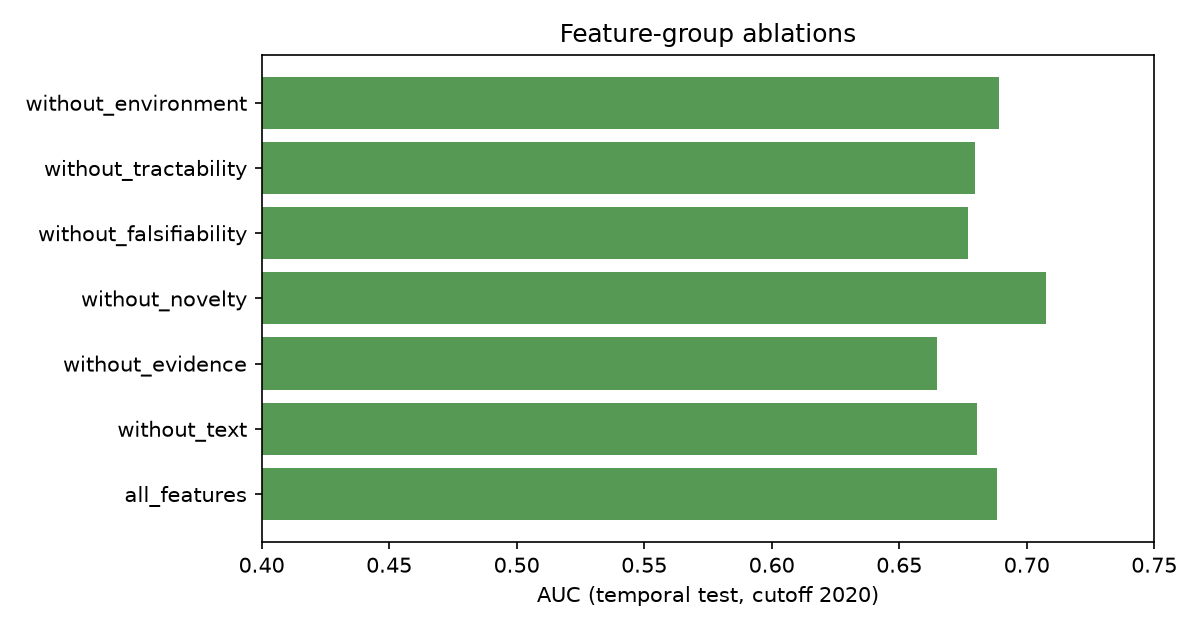
\includegraphics[width=0.85\linewidth]{ablations}
  \caption{Feature-group ablations (GBM, temporal test split).}
  \label{fig:ablations}
\end{figure}

\subsection{Which properties robustly predict attention}
\label{sec:predictors}

Controlled logistic effects (standardized, with subfield + cutoff +
source + environment covariates), with sign-stability across the 5
cutoffs / 8 subfields / 4 sources, are given in
Table~\ref{tab:predictors} and Figure~\ref{fig:predictor-effects}.

\begin{table}[htbp]
  \centering
  \caption{Controlled effects on future attention with sign-stability
  fractions across cutoffs / subfields / sources.}
  \label{tab:predictors}
  \footnotesize
  \setlength{\tabcolsep}{4pt}
  \begin{tabular}{lccc}
    \toprule
    Predictor & $\beta$ & $p$ & Sign-stable (cut./subf./src.) \\
    \midrule
    Review overlap (already visible in pre-cutoff reviews) & $\mathbf{+0.34}$ & $4\times10^{-5}$ & 1.00 / 0.88 / 1.00 \\
    N.\ directly similar prior papers                      & $\mathbf{+0.26}$ & 0.005            & 0.80 / 1.00 / 0.75 \\
    Instrument diversity of prior evidence                 & $\mathbf{-0.21}$ & 0.005            & 1.00 / 0.75 / 1.00 \\
    Explicit competing hypotheses (LLM-coded)              & $\mathbf{+0.17}$ & 0.021            & 0.80 / 0.88 / 0.50 \\
    Semantic novelty (distance to prior corpus)            & $+0.17$          & 0.030            & 1.00 / 0.75 / 0.50 \\
    Entity count                                           & $-0.17$          & 0.039            & 0.80 / 0.75 / 0.50 \\
    Specificity score                                      & $-0.16$          & 0.041            & 0.80 / 1.00 / 0.50 \\
    Evidence tension density                               & $+0.06$          & 0.52             & 0.60 / 0.62 / 0.50 \\
    \bottomrule
  \end{tabular}
\end{table}

\begin{figure}[htbp]
  \centering
  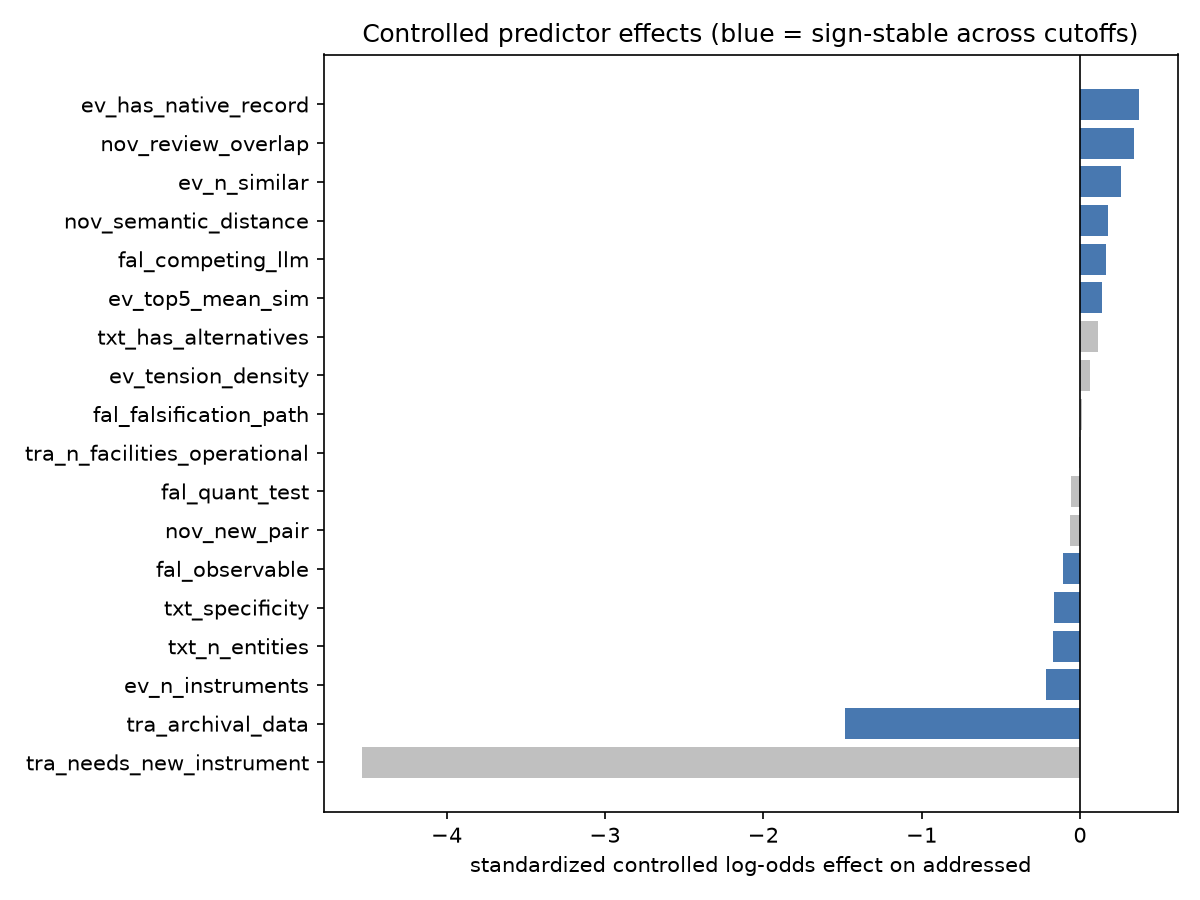
\includegraphics[width=0.85\linewidth]{predictor_effects}
  \caption{Controlled predictor effects on future attention.}
  \label{fig:predictor-effects}
\end{figure}

The picture that survives all four analyses:

\begin{enumerate}
  \item \textbf{The community mostly answers questions it has already
    begun to recognize.} Overlap with pre-cutoff reviews is the
    strongest, most stable predictor --- future attention is highly
    autocorrelated with present institutional attention, even after
    controlling for field size and growth.
  \item \textbf{A dense base of directly related evidence predicts
    uptake; evidence \emph{tension} per se does not.} What matters is
    that many papers already bear on the question, not that they
    disagree.
  \item \textbf{Questions whose evidence spans many instruments are
    \emph{less} likely to be engaged} --- consistent with
    multi-instrument questions being synthesis-level problems that no
    single group owns.
  \item \textbf{Explicitly articulated competing hypotheses help} ---
    the one falsifiability property with predictive teeth.
  \item \textbf{Specificity cuts against measured attention.} Highly
    entity-specific questions are engaged less often and \emph{more
    slowly} (Cox HR 0.73 per SD, $p<10^{-4}$) under literature-bounded
    labels --- partly a real narrowness effect, partly the retrieval
    bound (Section~\ref{sec:limitations}).
\end{enumerate}

\paragraph{Time-to-engagement (Task C).} In the Cox model (516
events/980), retrieval-similarity mass dominates speed (HR 3.77 per SD),
field growth accelerates engagement (HR 1.15), an explicit falsification
path accelerates it (HR 1.15), and specificity (HR 0.73) and tension
density (HR 0.88) slow it. Within-cell ranking of 2020 questions by
model score correlates with realized future paper counts at mean
Spearman $\rho = 0.29$ across the 8 test cells.

\paragraph{Outcome type (Task B).} The five-way status classifier
reaches macro-F1 0.23 (accuracy 0.56): it separates addressed/partial
from not-addressed but cannot yet learn the rare classes (8 answered,
4 refuted in total) --- exactly the sample-size regime the design
anticipated, and the reason Task A is primary at $n \approx 1{,}000$.

\subsection{Pre-stated hypotheses: mostly falsified}

\begin{table}[htbp]
  \centering
  \caption{Verdicts on the six pre-stated hypotheses.}
  \label{tab:hypotheses}
  \small
  \begin{tabular}{p{0.30\linewidth}p{0.62\linewidth}}
    \toprule
    Hypothesis & Verdict \\
    \midrule
    H1 tension $>$ novelty &
      \textbf{No.} Novelty carries a small positive controlled effect
      ($\beta=0.17$, $p=0.03$); tension density is null ($\beta=0.06$,
      $p=0.52$). \\
    H2 observation availability $\rightarrow$ attention &
      \textbf{No.} Operational-facility count is null on attention
      ($p=0.91$); refutation side untestable (4 cases). \\
    H3 competing hypotheses $\rightarrow$ answered &
      \textbf{Directionally yes, underpowered.} On attention:
      $\beta=0.17$, $p=0.02$. On answered-given-addressed:
      $\beta=0.56$, $p=0.08$. \\
    H4 novelty inverted-U &
      \textbf{No.} Quadratic term null ($p=0.46$). \\
    H5 popularity $\rightarrow$ counts, not answers &
      \textbf{Untestable as stated.} Count effect positive but n.s.\
      ($p=0.21$); answer side degenerate (8 answered). \\
    H6 tension $\times$ tractability interaction &
      \textbf{Marginal.} $\beta=0.16$, $p=0.053$ --- suggestive,
      unconfirmed. \\
    \bottomrule
  \end{tabular}
\end{table}

We regard this table as a feature of the method, not a failure of the
paper: five of six mechanism intuitions that sound compelling in a
proposal do not survive contact with a thousand historical outcomes and
proper controls.

\subsection{Interpretable prediction cards}

The released pipeline emits, for any frozen question, a card of the form:

\begin{quote}\small\ttfamily\raggedright
Question: How does the dark matter distribution in the innermost regions
of dwarf galaxies compare to the predictions of cold dark matter
simulations? [evidence\_tension, cutoff 2020]\\
Predicted P(future attention): 0.50 $\rightarrow$ observed: addressed
(partial)\\
Main positive factors: review overlap, directly similar prior papers,
explicit competing explanations\\
Main negative factors: high entity specificity, multi-instrument
evidence base
\end{quote}

A cautionary card from the Paper 1 import: \emph{``To what extent have
actual JWST observations validated pre-launch predictions that
aerosol-free TRAPPIST-1 CO$_2$ features should be detectable\ldots''}
(frozen at 2020-12-31, predicted 0.003, observed not addressed under our
retrieval). The phrase ``actual JWST observations'' presumes data that
did not exist at the cutoff --- an instance of generation-time knowledge
contaminating the \emph{phrasing} of a nominally frozen question. Every
LLM-mediated pipeline, including ours and Paper 1's, needs phrasing
audits of exactly this kind --- Paper 2 v1.1's released curation log
institutionalizes them, recording presupposition and phrasing repairs
made before freezing --- and the dataset makes such audits possible
because provenance is stored verbatim.

\subsection{A learned prior over evidence-graph structures}
\label{sec:structureprior}

Paper 2's outlook section poses the question its architecture needs
answered next: \emph{which structural patterns of pre-cutoff evidence
most often lead to questions the future answers, advances, or refutes?}
Our dataset can answer it empirically, because every tension-mined
question stores its generating evidence cluster verbatim --- sentences,
arXiv ids, dates. We derive a structural feature record for all 374
tension questions with the same transparent rules used elsewhere in the
pipeline (\texttt{pipeline/structure.py}; frozen in
\texttt{data/features/structure\_features\_v1.jsonl}): cluster breadth
(papers and claims in tension), evidence-age profile, a four-way tension
typology (explicit contradiction, unexplained result, methodological
challenge, detection-vs-limit stance opposition), quantification of the
discrepancy ($N$-sigma / factor-of markers), instrument structure, and
\textbf{recurrence} --- whether the same tension (shared source papers,
same subfield) was already detectable at an earlier cutoff, a
cutoff-time property since earlier past-windows are subsets of the
current one. Table~\ref{tab:structure} and
Figure~\ref{fig:structure-prior} summarize the indicators.

\begin{table}[htbp]
  \centering
  \caption{Evidence-graph structure indicators on the 374 tension
  questions. Controlled effects include subfield, cutoff, and
  environment covariates.}
  \label{tab:structure}
  \small
  \begin{tabular}{lcc}
    \toprule
    Structure indicator & Addressed rate & Controlled effect on addressed \\
    \midrule
    4-paper cluster (vs.\ 2--3-paper) & 0.54 vs.\ 0.32 & $\beta=\mathbf{+0.45}$/SD, $p=0.001$ \\
    Explicit contradiction markers    & 0.49 vs.\ 0.28 & $\beta=\mathbf{+0.30}$, $p=0.014$ \\
    Unexplained-result markers        & 0.49 vs.\ 0.43 & $+0.19$, $p=0.10$ \\
    Methodological challenge          & 0.46           & $-0.11$, n.s.; 0/61 resolved \\
    Quantified tension ($N$-$\sigma$) & 0.48           & null; carries all 3 refutations \\
    Recurrent across cutoffs          & 0.49           & null; carries all 6 resolutions \\
    \bottomrule
  \end{tabular}
\end{table}

\begin{figure}[htbp]
  \centering
  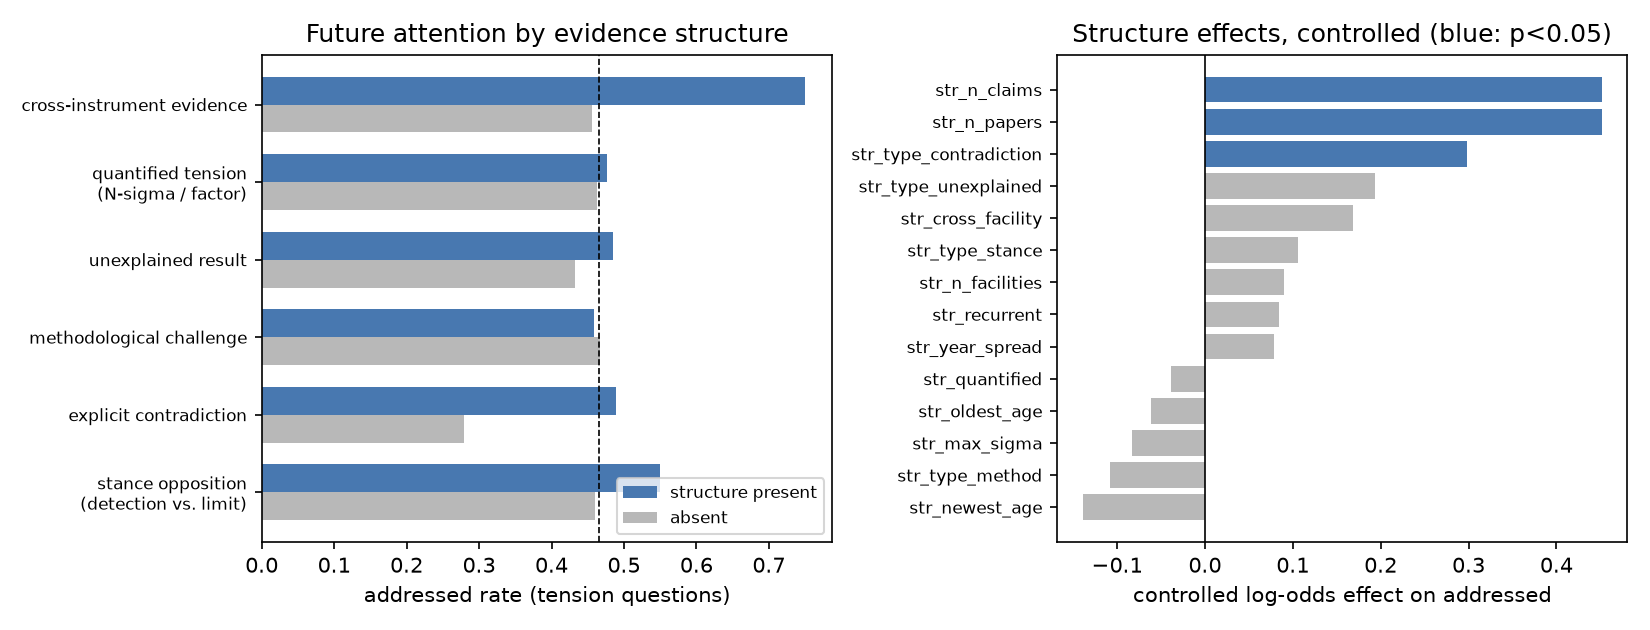
\includegraphics[width=\linewidth]{structure_prior}
  \caption{Evidence-graph structure and future attention. Left:
  addressed rates with each structure present vs.\ absent (dashed line:
  tension-question base rate). Right: controlled log-odds effects
  (blue: $p<0.05$).}
  \label{fig:structure-prior}
\end{figure}

Three structural regularities emerge, one per outcome layer:

\begin{enumerate}
  \item \textbf{Breadth buys attention.} The number of independent
    papers already in tension is the strongest structural predictor of
    both being addressed (0.54 for 4-paper clusters vs.\ 0.32 for
    2--3-paper, Fisher $p=6\times10^{-5}$) and future paper volume
    ($\beta=+0.12$, $p=0.03$) --- the structure-level counterpart of
    the question-level ``density of directly related prior evidence''
    predictor of Section~\ref{sec:predictors}. Fresher evidence also draws more future
    papers (evidence age on volume: $\beta=-0.17$, $p=0.002$).
  \item \textbf{Explicit contradiction buys engagement; methodological
    doubt does not resolve.} Clusters whose sentences explicitly
    disagree are addressed at 0.49 vs.\ 0.28 without such markers
    ($p=0.0095$), and five of the six resolved cases are
    contradiction-typed. Clusters built on methodological-challenge
    language engage the community at the average rate but resolved
    nothing (0/61) --- consistent with Paper 2's finding that questions
    must aim at a contestable claim, not at a diffuse worry about
    methods.
  \item \textbf{Quantification and persistence mark the refutation
    channel.} All three premise refutations come from
    \emph{quantified} clusters (3/63 vs.\ 0/311 unquantified, Fisher
    $p=0.005$), and all six resolutions come from \emph{recurrent}
    tensions (6/194 vs.\ 0/180 first-seen, $p=0.03$) --- structures the
    miner found again at two or more successive cutoffs. One honesty
    note bounds this: the three refutations trace to a single physical
    case (the FRB Galactic-latitude detection-rate discrepancy,
    independently re-mined at the 2016, 2018, and 2020 cutoffs and
    refuted by the same 2021 study), so they constitute one independent
    refutation event, and we report this layer as a case-level
    observation, not a statistical claim. Its shape is nonetheless
    exactly what Paper 2's protocol predicts: a persistent, quantified,
    explicitly contradictory tension is a published conclusion waiting
    to be overturned.
\end{enumerate}

The prior is learnable and transfers out of time: a logistic model on
structural features alone, trained on the 2012--2018 cutoffs, ranks
2020 tension questions at AUC 0.586 ($n=80$) --- modest in absolute
terms, but notable against the right comparison: restricted to the same
single-source subset, the full 50-feature question-level record manages
only AUC 0.502, because most of its cross-source signal is generator
style and topic hotness that vanish within one source. Within a single
generator, the generating \emph{structure} is the recoverable signal.
And because every structural feature is computable at mining time ---
before any question is phrased --- the fitted coefficients
(\texttt{results/structure\_prior.json}) constitute a ranking prior for
exactly the machine-scale structural search Paper 2's outlook proposes:
enumerate candidate tensions, rank by breadth, explicit contradiction,
quantification, and persistence, verbalize the survivors. The
prospective instance (Section~\ref{sec:conclusion}) is the pre-registered test of whether
this prior holds on a future no model has seen.

\subsection{Robustness, calibration, and the label-noise ceiling}
\label{sec:robustness}

Four analyses probe how much of the above depends on analytic choices, and
what the measured label noise implies about the best any model could do
(\texttt{results/robustness.json}; all computed from the frozen records).

\paragraph{The engagement bar.} The released label derives
\texttt{addressed} from at least one \emph{direct} future candidate. Under
stricter bars the levels drop, but the contrast that carries the leakage
claim survives every bar, while the tension-vs-control contrast weakens
into noise (Table~\ref{tab:bars}). At $n_\mathrm{direct}\geq 3$ tension
questions sit nominally below controls (0.115 vs.\ 0.140), a crossover
that is not significant ($p=0.43$) and whose composition is diagnostic:
22 of the 28 controls clearing that bar are of the \emph{vague} subtype.
Vague questions accumulate ``direct'' hits because breadth makes the
direct/adjacent distinction permeable, whereas engaged tension questions
are engaged \emph{thinly} --- 1.9 direct papers on average, with 75\% at
one or two, against 3.2 and 42\% for direct-LLM questions --- and
$n_\mathrm{direct}$ correlates negatively with entity count
($\rho=-0.12$) and specificity ($\rho=-0.17$, both $p<10^{-3}$). The
strict-bar crossover is thus the specificity effect and the
breadth-farming failure mode meeting in one number, not a reversal of
question quality.

\begin{table}[htbp]
  \centering
  \caption{Addressed rate under stricter direct-engagement bars. Fisher
  $p$ against controls.}
  \label{tab:bars}
  \small
  \begin{tabular}{lcccccc}
    \toprule
    Bar & All & Controls & Tension & Direct LLM & LLM vs.\ ctrl & Tension vs.\ ctrl \\
    \midrule
    $n_\mathrm{direct}\geq 1$ & 0.527 & 0.320 & 0.465 & 0.880 & $p<10^{-4}$ & $p=0.0007$ \\
    $n_\mathrm{direct}\geq 2$ & 0.333 & 0.185 & 0.238 & 0.685 & $p<10^{-4}$ & $p=0.17$ \\
    $n_\mathrm{direct}\geq 3$ & 0.212 & 0.140 & 0.115 & 0.515 & $p<10^{-4}$ & $p=0.43$ \\
    \bottomrule
  \end{tabular}
\end{table}

\paragraph{Retrieval bound and uncertainty.} The stored top-8 similarity
lists quantify how retrieval-bounded the labels are: at the released
threshold ($\tau=0.18$) 40\% of questions already have no candidate above
threshold, rising to 67\% at $\tau=0.22$ --- the ``lower bound'' caveat in
numbers. Bootstrap intervals (2{,}000 resamples) put the headline
addressed rate at 0.527 [0.496, 0.557] and the non-control-minus-control
gap at 0.259 [0.180, 0.330]. The judge's self-reported confidence is
itself informative about its behaviour: it assigns full confidence chiefly
when rejecting (addressed rate 0.235 at confidence 1.0 vs.\ 0.867 at 0.9),
i.e.\ it is certain about absence and hedges about presence.

\paragraph{The label-noise ceiling.} The independent second judge agrees
with the primary on \texttt{addressed} 63.5\% of the time. Modelling both
as independent, class-symmetric noisy readers of a latent truth, that
agreement implies a per-judge flip rate of 0.24 --- and a \emph{perfect}
oracle for the latent truth would score only \textbf{AUC 0.758} against
the primary labels. The observed temporal-split AUC of 0.713 is then
\textbf{83\% of the achievable range above chance}. The split of the
measured disagreement between the judges is not identified --- attributing
more of it to the second judge raises the ceiling (to 0.90 if the primary
judge's flip rate is 0.10) --- but under any allocation the ceiling sits
well below 1: raw AUC materially understates predictive skill on
noisy-labelled outcomes, a point that applies to any study scoring
open-ended outcomes with an imperfect judge.

\paragraph{Calibration and errors.} Discrimination is not calibration:
the temporal-split logistic model reaches Brier 0.224 with
quintile-binned ECE 0.109, well calibrated at the extremes (top bin:
predicted 0.87, observed 0.86) and overconfident in the middle (predicted
0.59, observed 0.45; Figure~\ref{fig:calibration}). Its false positives
do not show inflated review overlap relative to true negatives (0.077
vs.\ 0.075), so the strongest predictor is not the failure mode. The
most instructive error is a false negative: the model's second-lowest
test-set prediction (0.089) is the HD~209458\,b water-abundance question
imported from~\cite{paper1} --- precisely the question the community
engaged by \emph{refuting its premise}. The attention model assigns near
zero to the dataset's clearest instance of a question doing what
questions are for, which is the sharpest single demonstration that
predicted attention and question value are different quantities
(Section~\ref{sec:theory}).

\begin{figure}[htbp]
  \centering
  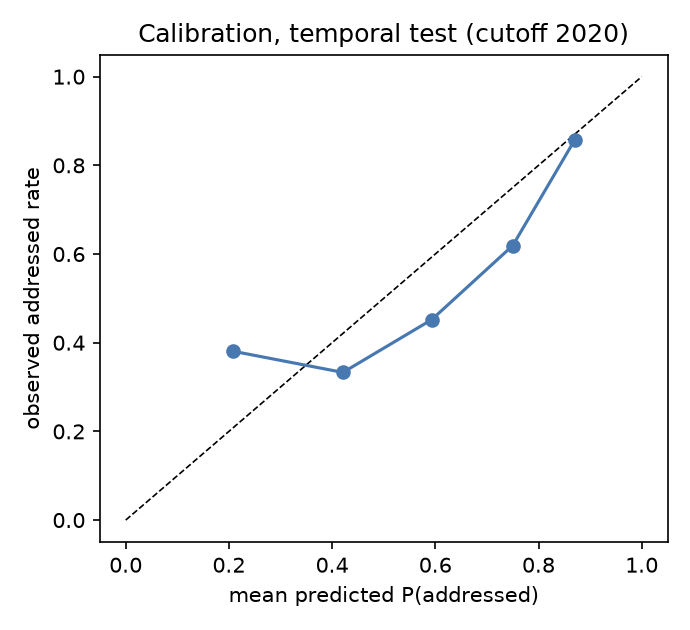
\includegraphics[width=0.6\linewidth]{calibration}
  \caption{Reliability diagram, temporal test split (quintile bins,
  $n=210$).}
  \label{fig:calibration}
\end{figure}

\subsection{Cross-domain replication: anti-aging skincare ingredients}
\label{sec:crossdomain}

Every conclusion so far rests on one science. To test which of them are
astronomy's, we ported the complete protocol --- unchanged where
possible, and changed only in directions this paper itself prescribes
--- to a maximally distant literature: anti-aging and anti-wrinkle
skincare-ingredient research. The corpus is the complete PubMed record
of English abstracts matching one reproducible skin-aging $\times$
ingredient query (19{,}193 papers, 2005--2026); the eight subfields
become twelve ingredient classes; the facility lexicon becomes an
assay-availability lexicon; and the same five cutoffs, past/future
windows, source mix (tension, future-work, weak/negative controls), six
feature groups, temporal and leave-one-class-out splits, pre-stated
hypotheses, and structural prior are applied to \textbf{1{,}043
backtested questions}. Two deliberate deviations implement this paper's
own v2 requirements (Section~\ref{sec:limitations}): questions are
verbalised by deterministic templates over verbatim pre-cutoff
sentences, removing the parametric-leakage channel entirely (no
language model is called at any stage), and the outcome judge is the
reliability-gated, checkable-condition rule our limitations section
calls for --- direct engagement requires retrieval relevance, an
anchor-ingredient match, and a skin-aging outcome term; \emph{answered}
requires a direct randomised trial or meta-analysis --- making every
label reproducible bit-for-bit.

The protocol transfers (Table~\ref{tab:crossdomain}). Future attention
is again predictable out-of-time (interpretable logistic AUC 0.746 on
the 2020 test cutoff, $n=226$; gradient boosting 0.836), again survives
training on the six mature ingredient classes and testing on the six
emerging ones (0.72--0.77), and again clears chance in every
leave-one-class-out split (0.67--0.93). Controls again land lowest
(26.8\% vs.\ 40.3\% for tension-mined questions), and the structural
breadth effect of Section~\ref{sec:structureprior} replicates in sign
and significance at about half the size ($\beta=+0.23$, $p=0.04$). All
six pre-stated hypotheses fail again: across the two domains, twelve
pre-registered mechanism tests now yield one directional survivor, H3,
marginal in both ($\beta=0.56$, $p=0.08$; $\beta=0.71$, $p=0.061$),
while astronomy's marginal H6 interaction does not replicate
($p=0.69$). Most tellingly, the reliability ceiling reappears under a
different kind of judge: a blinded second judgement of a stratified
sample gives 65.6\% raw agreement and $\kappa=0.22$ on
\emph{addressed} --- against 63.5\% and $\kappa=0.21$ here --- even
though the replication's primary judge is a deterministic rule rather
than a language model. The ceiling lives in the outcome taxonomy
itself, not in any particular judge, which is what the noise-ceiling
construction of Section~\ref{sec:robustness} assumes.

\begin{table}[htbp]
  \centering
  \caption{The protocol and its findings across the two domains.
  Absolute rates and AUCs are comparable only within one column (the
  instances differ in judge and recalibrated retrieval thresholds).}
  \label{tab:crossdomain}
  \footnotesize
  \setlength{\tabcolsep}{4pt}
  \begin{tabular}{lcc}
    \toprule
    & Astronomy (this paper) & Skincare replication \\
    \midrule
    Corpus & 313{,}189 arXiv astro-ph & 19{,}193 PubMed \\
    Backtested questions & 980 & 1{,}043 \\
    Verbalization & LLM (temp.\ 0, cached) & deterministic templates \\
    Outcome judge & blinded LLM rubric & checkable-condition rule \\
    Addressed: controls / tension & 0.32 / 0.47 & 0.27 / 0.40 \\
    Out-of-time AUC (interpretable / best) & 0.713 / 0.718 & 0.746 / 0.836 \\
    Held-out-domain AUC & 0.65--0.71 & 0.72--0.77 \\
    Evidence density $\beta$ & $+0.26$ & $+0.79$ \\
    Review overlap $\beta$ & $\mathbf{+0.34}$ & $0.00$ ($p=0.95$) \\
    Specificity $\beta$ (Cox HR/SD) & $-0.16$ (0.73) & $\mathbf{+0.57}$ (1.29) \\
    Competing hypotheses $\beta$ & $+0.17$ & $+0.28$ \\
    Evidence tension density $\beta$ & $+0.06$ (n.s.) & $-0.09$ (n.s.) \\
    Hypotheses supported & 0/6 (H3 marginal) & 0/6 (H3 marginal) \\
    Structural breadth $\beta$ & $+0.45$, $p=0.001$ & $+0.23$, $p=0.04$ \\
    Second-judge agreement ($\kappa$) & 63.5\% (0.21) & 65.6\% (0.22) \\
    \bottomrule
  \end{tabular}
\end{table}

What does \emph{not} transfer is as informative as what does, because
the changes go in the directions the theoretical framework predicts
rather than in random ones. Exactly one predictor is sign-stable across
every cutoff, class, and source \emph{in both domains}: the density of
directly similar prior evidence ($\beta=+0.26$ here, $+0.79$ there) ---
the quantity Section~\ref{sec:theory} identifies with amortised
evaluation cost, and the framework's central prediction. The
recognition cue it rides on, however, is domain-specific: review
overlap, astronomy's strongest predictor, is exactly null in the
ingredient literature ($\beta=0.00$, $p=0.95$), displaced by naming a
specific ingredient ($\beta=+0.76$) --- in a field organised around
named actives rather than named objects, the ingredient name \emph{is}
the recognition handle. (The effect is partly instrumental, since the
rule judge anchors on ingredient names; the retrieval-bound caveat of
Section~\ref{sec:discussion} applies with its sign flipped.) Most
strikingly, specificity reverses sign: negative and decelerating in
astronomy ($\beta=-0.16$; Cox HR 0.73/SD), it is a strong positive
predictor in skincare ($\beta=+0.57$, $p<10^{-10}$) that
\emph{accelerates} engagement (HR 1.29, $p=2\times10^{-4}$). The
foraging account prices the reversal in engagement cost: a specific
ingredient claim can be tested by one vehicle-controlled twelve-week
split-face trial, so specific questions are cheap, high-yield patches;
a specific astronomy claim needs scheduled telescope time that no group
can allocate around one question. Where acting on a question is cheap,
specificity is a yield cue; where it is expensive, specificity narrows
the addressable community. A theory of attention allocation whose cue
weights could \emph{not} change across domains with different cost
structures would be wrong about its own mechanism; this one changes
them in the observed direction while keeping its central quantity
fixed. Evidence tension, meanwhile, is null in both domains ($+0.06$
and $-0.09$): the H1 failure is not an astronomy accident.

Three caveats keep the comparison honest. The two instances differ in
judge and in recalibrated retrieval thresholds, so absolute rates and
AUCs are comparable only within one instance --- the lesson of
Section~\ref{sec:pipeline} applied to ourselves. The replication's
refutation channel is empty (its two premise-challenged cases were both
unconfirmed by the second judge and are treated as absent), so the
refutation-side structural indicators could not be re-tested. And the
rule judge's \emph{answered} (``a direct trial or meta-analysis
exists'') is measurably more lenient than a human ``settled'': six of
eight audited \emph{answered} cases were downgraded to partial. The
replication's full pipeline, frozen questions, features, labels, audit
verdicts, and result tables are released alongside this paper's.

\section{Discussion}
\label{sec:discussion}

\paragraph{What the dataset says about question value.} The strongest
honest summary: five-year scientific attention is predictable to a
useful degree (AUC $\sim$0.7 out-of-time and out-of-domain) from
cutoff-time properties, but the predictive properties are about the
question's \emph{relationship to its community} --- already-in-reviews,
dense direct evidence, articulated alternatives --- more than about the
intrinsic virtues the literature on ``good questions'' celebrates
(novelty, tension, specificity). Attention follows preparation ---
the behaviour the recognition-constrained foraging account of
Section~\ref{sec:theory} predicts and explains. Whether
that is how science \emph{should} allocate attention is precisely the
kind of question this dataset now lets others study: the rare
premise-refuted cases, the slow-burning specific questions, and the
unaddressed-but-well-formed tail are all released with full provenance.

\paragraph{Specificity and the measurement bound.} The negative
specificity effect is partly real (narrow questions have small
addressable communities) and partly instrumental: abstract-level TF--IDF
retrieval misses engagement with object-level questions, as the Paper 1
subset demonstrates (2/10 here vs.\ 10/10 under Paper 2's full-text
evaluation). We report it as ``less \emph{measured} attention'', never
``worse questions'' --- and this is the main reason Task A labels should
be read as lower bounds. Paper 2 v1.1 attacks the same confound from
the metric side with a specificity-adjusted foresight score that
down-weights broad questions anything would engage; under that rubric
object-anchored questions are precisely what makes outcomes
\emph{resolvable} (its structure-first pipelines, 95--100\%
object-anchored, refute premises in every era; its LLM-only pipeline,
5\% anchored, refutes almost none). The two results agree that raw
engagement over-rewards breadth and under-rewards specificity; they
differ only in the remedy --- adjust the metric (Paper 2) versus
control and caveat in the regression (here).

\paragraph{The direct-LLM anomaly is a warning, not a victory.} The 88\%
addressed rate for direct-LLM questions is exactly what parametric
leakage would produce: a model asked in hindsight for ``the most
important open questions of 2016'' can simply recall what 2017--2021
worked on. Because source is a covariate in every regression, the
predictor analysis is shielded from this; but any future benchmark that
scores generators by addressed-rate alone will be gamed by hindsight
knowledge. Mined sources with verbatim pre-cutoff provenance are the
defensible foundation. Paper 2 v1.1's generator decomposition and
temporal stress test now make this point causally rather than
suggestively: over identical pre-cutoff evidence structures, a
weight-free structural generator finds engaged questions in every era,
the LLM adds value only as a separable verbalization layer, and the
LLM-only pipeline's performance never rested on specifics that
memorization could supply --- its answered rate is flat across the
model's training boundary because a topic prior needs no memory of the
future. Our regression-level shielding (source as a covariate in every
model) and Paper 2's decomposition are complementary defenses against
the same threat, operating at the analysis and generation levels
respectively.

\paragraph{Implications for system design.} The findings convert into
three concrete practices. For \emph{generator architectures}, they
select an ordered pipeline: enumerate candidate evidence tensions at
machine scale; rank them by the mining-time structure prior of
Section~\ref{sec:structureprior} --- cluster breadth, explicit
contradiction, quantification, cross-cutoff persistence --- and
verbalise only the survivors, since phrasing adds resolution but no
foresight~\cite{paper2}. Every ranking feature is computable before a
question is written, so the prior adds no generation-time cost. For
\emph{evaluation design}, three practices transfer to any
engagement-scored benchmark: include deliberately weak controls so that
chance has a measured price (here pure chance costs 8.7\%, not zero);
price vagueness explicitly, because the worst-by-construction questions
game coverage in practice and not only in principle
(Table~\ref{tab:subtypes}); and publish judged metrics only alongside
measured reliability and the noise ceiling it implies, without which an
AUC or an addressed rate cannot be interpreted. For
\emph{recommendation}, the two strongest predictors --- prior
recognition and evidence density --- are computable from a live corpus,
so a research assistant could rank candidate questions by predicted
uptake today. That capability carries a Goodhart warning the framework
makes precise: predicted attention as an optimisation target would
amplify exactly the conservatism it measures, recommending the
already-recognised and making recognition self-fulfilling. A deployment
that cares about value rather than popularity should pair the attention
model with the refutation-channel indicators --- quantified, persistent
contradictions --- which point at overturnable conclusions rather than
at the crowd's path.

\section{Limitations}
\label{sec:limitations}

\begin{itemize}
  \item \textbf{Abstract-level corpus.} Full texts are not used; tension
    and future-work mining see only abstracts, and citation-weighted
    attention is unavailable without a second data provider. Paper
    counts, lead times, and review recognition stand in for citation
    impact.
  \item \textbf{Retrieval-bounded labels.} A question can be engaged by
    literature our TF--IDF retrieval misses; not\_addressed is a lower
    bound on engagement, uniformly across sources but not uniformly
    across specificity (see Section~\ref{sec:discussion}).
  \item \textbf{LLM judges, not humans.} Label reliability is estimated
    with an independent second model rather than human adjudication
    (63.5\% raw agreement, $\kappa=0.21$, disagreement one-directionally
    lenient). Paper 2 v1.1's seven-rater study reframes what such
    numbers can mean: on the analogous taxonomy, two independent human
    annotators agreed with each other at only $\kappa=0.17$, every
    judge model matched the professional annotator as well as or better
    than the humans matched each other, and model--model agreement
    ($\kappa$ up to 0.60) would have overstated reliability threefold.
    The weakness lives in outcome taxonomies of this kind, not in our
    judge specifically; accordingly, absolute rates here are
    rater-relative, all comparative results hold the judge fixed, and a
    reliability-gated taxonomy (fewer labels, checkable conditions, a
    measured human--human $\kappa$ before release) is the shared v2
    requirement for both papers. The annotation protocol, rationales,
    and supporting ids are released so human passes can replace or
    audit the judges; per-class precision tables are in the released
    agreement report.
  \item \textbf{Parametric-knowledge leakage.} The direct-LLM source
    (and, weakly, LLM phrasing of mined material) can import post-cutoff
    knowledge despite freeze instructions --- including into question
    phrasing, as the JWST card shows. Source is controlled for in all
    analyses; the direct-LLM addressed rate should not be read as
    generator quality.
  \item \textbf{Rare outcomes remain rare.} 8 answered and 4
    premise-refuted questions cannot support the Task B taxonomy or
    H2/H5 as stated; the design document's projection that these classes
    need 2{,}000--5{,}000 questions is confirmed empirically.
  \item \textbf{The noise ceiling is model-based.} The AUC ceiling of
    Section~\ref{sec:robustness} assumes class-symmetric, independent
    judge errors, and neither assumption is innocent. Both judges read
    the same retrieved candidates, so their errors are plausibly
    positively correlated; for a fixed observed agreement that implies
    \emph{more} per-judge noise and a \emph{lower} true ceiling than
    reported, making the 83\% skill fraction conservative. Asymmetric
    class errors cut the other way. The scan over error splits bounds
    the leverage of the symmetric assumption, but only human
    adjudication could replace the model with a measurement.
  \item \textbf{Two domains, one primary.} The full analysis is
    astronomy's; the skincare-ingredient replication
    (Section~\ref{sec:crossdomain}) shows the protocol and the
    evidence-density predictor transfer, but it uses a different judge,
    its refutation channel is empty, and two domains do not span
    science. Fields whose engagement-cost structure differs from both
    --- mathematics, say, where acting on a question is neither a trial
    nor an observation --- remain open.
\end{itemize}

\section{Conclusion}
\label{sec:conclusion}

We built the first temporally grounded, multi-cutoff, multi-source
dataset of scientific questions with future-outcome labels, and used it
to replace two common practices: scoring questions by how they sound,
and validating question generators on single-digit case studies. At
$n=980$ with strict blinded labeling, future scientific attention is
predictable (AUC $\approx 0.71$ out-of-time and out-of-domain, and
0.75--0.84 in an independent second-domain replication) --- and
the robust predictors are community-relational, not rhetorical. That
number is 83\% of the ceiling measured label noise permits, and the
predictors are exactly those a recognition-constrained foraging account
of attention allocation selects (Section~\ref{sec:theory}); the
ceiling construction itself transfers to any study that scores
open-ended outcomes with an imperfect judge. Most
pre-registered mechanism hypotheses failed, which is the point: a
dataset an order of magnitude larger than its predecessor makes
intuitions testable, and most did not survive. The dataset, every
prompt, every judge rationale, and the full pipeline are released for
the community to reuse, audit, and extend to other sciences --- and the
skincare-ingredient replication of Section~\ref{sec:crossdomain} shows
that the extension is a port, not a rebuild: the protocol, the
evidence-density predictor, the hypothesis failures, and the
reliability ceiling all reproduce in a second science, with the sign
flips the engagement-cost account predicts. An extension to a third
domain with harder outcome signals is in preparation (clinical
oncology, where trial registrations and phase transitions are
observable events rather than retrieval-bounded labels). A
forward-looking test is already armed: Paper 2 v1.1's prospective
instance --- 200 questions from four generators, frozen 2026-08-17 with
a pre-registered 2027--2030 scoring window --- will let the predictors
learned here be evaluated against a future no model has seen,
converting this paper's retrospective claims into ones that time itself
will grade.

\section*{Reproducibility}

All code, the frozen dataset, labels, and results are released; every
pipeline stage is a single script, all LLM calls are cached and pinned
to temperature 0, and the offline test suite plus a temporal-isolation
validator run in CI. Rebuilding the corpus from the public arXiv API and
regenerating the dataset reproduced the frozen questions byte-for-byte.
The frozen dataset is additionally published on the Hugging Face Hub at
\href{https://huggingface.co/datasets/huiluckylucky/scientific-question-outcomes}{\texttt{huiluckylucky/scientific-question-outcomes}},
loadable in one call, with the structure-prior and second-judge subsets as
separate configurations.
The cross-domain replication of Section~\ref{sec:crossdomain} is
released as a separate repository with the same layout --- code, frozen
questions, features, labels, audit verdicts, and result tables --- at
\href{https://github.com/nonameisready/scientific-discovery-anti-age-integredients}{\texttt{nonameisready/scientific-discovery-anti-age-integredients}};
given its harvest, every replication number is deterministic (no
language-model calls at any stage).

\section*{Declaration of generative AI and AI-assisted technologies in the
writing process}

During the preparation of this work the author used Claude (Anthropic) to
draft and edit manuscript prose, to typeset the manuscript in \LaTeX, and to
assist in writing the analysis code for the evidence-structure prior
(\texttt{pipeline/structure.py} and \texttt{scripts/run\_structure\_prior.py}
in the released repository). After using this tool, the author reviewed and
edited the content as needed and takes full responsibility for the content of
the publication.

Separately, and as a matter of method rather than of manuscript preparation,
large language models are a component of the study itself: they phrase the
mined questions and assign the outcome labels. Their role, model versions,
prompts, and cached outputs are specified in Sections~3.2 and~3.4 and
released in full with the dataset.

\begin{thebibliography}{99}

\bibitem{baek2024}
Jinheon Baek, Sujay Kumar Jauhar, Silviu Cucerzan, and Sung Ju Hwang.
ResearchAgent: Iterative Research Idea Generation over Scientific Literature
with Large Language Models. arXiv:2404.07738, 2024.

\bibitem{bailey2014}
David H. Bailey, Jonathan M. Borwein, Marcos L\'opez de Prado, and Qiji Jim
Zhu. Pseudo-Mathematics and Financial Charlatanism: The Effects of Backtest
Overfitting on Out-of-Sample Performance. \emph{Notices of the American
Mathematical Society}, 61(5):458--471, 2014.

\bibitem{fortunato2018}
Santo Fortunato, Carl T. Bergstrom, Katy B\"orner, James A. Evans, Dirk
Helbing, Sta\v{s}a Milojevi\'c, Alexander M. Petersen, Filippo Radicchi,
Roberta Sinatra, Brian Uzzi, Alessandro Vespignani, Ludo Waltman, Dashun
Wang, and Albert-L\'aszl\'o Barab\'asi. Science of science.
\emph{Science}, 359(6379):eaao0185, 2018.

\bibitem{foster2015}
Jacob G. Foster, Andrey Rzhetsky, and James A. Evans. Tradition and
Innovation in Scientists' Research Strategies. \emph{American Sociological
Review}, 80(5):875--908, 2015.

\bibitem{hindsight2026}
Bo Jiang. HindSight: Evaluating LLM-Generated Research Ideas via Future
Impact. arXiv:2603.15164, 2026.

\bibitem{jimenez2024}
Carlos E. Jimenez, John Yang, Alexander Wettig, Shunyu Yao, Kexin Pei, Ofir
Press, and Karthik Narasimhan. SWE-bench: Can Language Models Resolve
Real-World GitHub Issues? In \emph{International Conference on Learning
Representations}, 2024.

\bibitem{kitano2021}
Hiroaki Kitano. Nobel Turing Challenge: creating the engine for scientific
discovery. \emph{npj Systems Biology and Applications}, 7:29, 2021.

\bibitem{landis1977}
J. Richard Landis and Gary G. Koch. The Measurement of Observer Agreement
for Categorical Data. \emph{Biometrics}, 33(1):159--174, 1977.

\bibitem{lu2024}
Chris Lu, Cong Lu, Robert Tjarko Lange, Jakob Foerster, Jeff Clune, and
David Ha. The AI Scientist: Towards Fully Automated Open-Ended Scientific
Discovery. arXiv:2408.06292, 2024.

\bibitem{merton1968}
Robert K. Merton. The Matthew Effect in Science. \emph{Science},
159(3810):56--63, 1968.

\bibitem{pirolli1999}
Peter Pirolli and Stuart K. Card. Information Foraging.
\emph{Psychological Review}, 106(4):643--675, 1999.

\bibitem{rzhetsky2015}
Andrey Rzhetsky, Jacob G. Foster, Ian T. Foster, and James A. Evans.
Choosing experiments to accelerate collective discovery. \emph{Proceedings
of the National Academy of Sciences}, 112(47):14569--14574, 2015.

\bibitem{si2024}
Chenglei Si, Diyi Yang, and Tatsunori Hashimoto. Can LLMs Generate Novel
Research Ideas? A Large-Scale Human Study with 100+ NLP Researchers.
arXiv:2409.04109, 2024.

\bibitem{ideationgap2025}
Chenglei Si, Tatsunori Hashimoto, and Diyi Yang. The Ideation--Execution
Gap: Execution Outcomes of LLM-Generated versus Human Research Ideas.
arXiv:2506.20803, 2025.

\bibitem{simon1955}
Herbert A. Simon. A Behavioral Model of Rational Choice. \emph{Quarterly
Journal of Economics}, 69(1):99--118, 1955.

\bibitem{swanson1986}
Don R. Swanson. Fish Oil, Raynaud's Syndrome, and Undiscovered Public
Knowledge. \emph{Perspectives in Biology and Medicine}, 30(1):7--18, 1986.

\bibitem{uzzi2013}
Brian Uzzi, Satyam Mukherjee, Michael Stringer, and Ben Jones. Atypical
Combinations and Scientific Impact. \emph{Science}, 342(6157):468--472,
2013.

\bibitem{wang2021}
Dashun Wang and Albert-L\'aszl\'o Barab\'asi. \emph{The Science of Science}.
Cambridge University Press, 2021.

\bibitem{wang2024}
Qingyun Wang, Doug Downey, Heng Ji, and Tom Hope. SciMON: Scientific
Inspiration Machines Optimized for Novelty. In \emph{Proceedings of the 62nd
Annual Meeting of the Association for Computational Linguistics}, 2024.

\bibitem{zheng2023}
Lianmin Zheng, Wei-Lin Chiang, Ying Sheng, Siyuan Zhuang, Zhanghao Wu,
Yonghao Zhuang, Zi Lin, Zhuohan Li, Dacheng Li, Eric P. Xing, Hao Zhang,
Joseph E. Gonzalez, and Ion Stoica. Judging LLM-as-a-Judge with MT-Bench and
Chatbot Arena. In \emph{Advances in Neural Information Processing Systems},
2023.

\bibitem{zou2022}
Andy Zou, Tristan Xiao, Ryan Jia, Joe Kwon, Mantas Mazeika, Richard Li, Dawn
Song, Jacob Steinhardt, Owain Evans, and Dan Hendrycks. Forecasting Future
World Events with Neural Networks. In \emph{Advances in Neural Information
Processing Systems}, 2022.

\bibitem{paper1}
Hui Mao.
\emph{Evidence-Based Scientific Question Discovery: A Framework with
Historical Backtesting}.
arXiv:2608.09968, 2026.
\url{https://arxiv.org/abs/2608.09968}.
Referred to as ``Paper 1'' throughout.

\bibitem{paper2}
Hui Mao.
\emph{Historical Backtesting for Scientific Question Discovery: A
Protocol and Astronomy Pilot}.
arXiv:2608.16795 (v1.1, sealed), 2026.
\url{https://arxiv.org/abs/2608.16795}.
Referred to as ``Paper 2'' throughout.

\end{thebibliography}

\end{document}
